\section{Konzept zur Datenerfassung und - auswertung}
\label{concept}
Ein weiteres wichtiges Thema dieser Arbeit soll es sein, ein erstes Konzept zur automatischen Datenerfassung und - auswertung der nötigen Parameterdaten zu entwickeln. Dieses kann dann als Vorlage für einen Prototypen zur automatischen Einschätzung der Fahrtauglichkeit eines Fahrers vor Fahrtantritt dienen. Der grundlegende Entwurf ist in der Abbildung \ref{fig:conceptfmc} als FMC-Modell dargestellt.

\begin{figure}
	\centering
	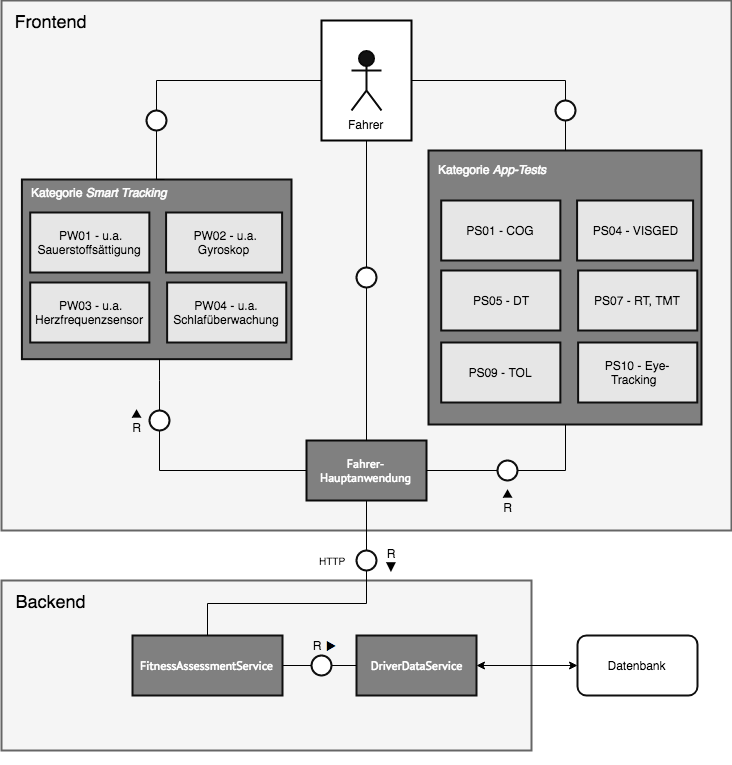
\includegraphics[width=\linewidth]{images/ConceptDriverAssessmentData}
	\caption[Caption for concept]{FMC-Modell der grundlegenden Anwendung}
	\label{fig:conceptfmc}
\end{figure}

Initiativ kann die Anwendung, z.B. in Form einer Smartphone-App, manuell durch den Nutzer gestartet werden. Die Anwendung \textit{Texive} von Bo et al. hat jedoch auch gezeigt, dass automatisch erkannt werden kann, wenn sich der Fahrer im Fahrzeug befindet \cite{texive}. Ein denkbares Szenario wäre hier, dass die Lenkradsperre erst gelöst wird, wenn etwaige App-Tests (Kategorie App-Tests) auf dieser Anwendung erfolgreich absolviert werden. Dieses Szenario bringt jedoch Probleme mit sich, welche im Anschluss diskutiert werden. Realistischer wäre hierbei eher, dass die Hauptanwendung die körperlichen Fahrerdaten permanent aus gekoppelten  Wearables speichert und im Falle des Fahrtantritts auswertet. Abbildung \ref{fig:conceptfmc} zeigt hier die Vorgehensweise. Die Hauptanwendung als Teil des Frontends schickt die gebündelten Fahrerdaten aus beiden Parameter-Kategorien an das Backend. Es wird an dieser Stelle offen gelassen, ob die Auswertung der Daten auf dem Smartphone direkt oder auf einem separaten Server vorgenommen wird.

Idealerweise übernimmt dann ein eigenständiger Dienst, in Abbildung \ref{fig:conceptfmc} als \textit{FitnessAssessmentService} betitelt, die eigentliche Evaluation der Fahrerdaten. Für die Kategorie App-Tests werden hier die Test-Ergebnisse genommen. Eine hohe Punktzahl entspräche einer guten Fahrtauglichkeit. Bei der Kategorie Smart Tracking müsste noch evaluiert werden, inwieweit die einzelnen Parameter beim Fahrer ausgeprägt sein müssen, um Fahrtauglichkeit nachzuweisen. Die Anwendung \textit{DriveSafe} von Bergasa et al. hat ein Punktesystem vorgestellt, in welchem das Fahrverhalten bewertet wird \cite{drivesafe}. Aufbauend auf diesem könnte man eine ähnliche Bewertung der körperlichen Verfassung auf Grundlage der Fahrerdaten vornehmen. 

Denkbar wäre zudem, die Fahrerdaten dauerhaft zu persistieren. Somit können Zustandsmuster des Fahrers auf lange Hinsicht untersucht werden, um so ebenfalls Aussagen über die Verfassung des Fahrers zu treffen. Hilfreich wäre dies u.a. bei Parameter \textit{PW04}, um eine auffällige Müdigkeit des Fahrers zu erkennen. Außerdem könnte für \textit{PW01} eine dauerhaft schlechte körperliche Verfassung erfasst werden. Die Persistenz-Vorgänge sollten dann über einen weiteren Dienst im Backend vorgenommen werden, auf welchem der \textit{FitnessAssessmentService} zugreifen könnte, um die nötigen Fahrerdaten dauerhaft zu erhalten. Dieser wird in Abbildung \ref{fig:conceptfmc} als \textit{DriverDataService} gekennzeichnet.

Letztendlich sendet der \textit{FitnessAssessmentService} eine abschließende Einschätzung der Fahrtauglichkeit an die Hauptanwendung. Denkbar wäre hier wieder, dass nur bei positivem Ergebnis das Lenkrad des Fahrzeugs entsperrt wird. 
